\section {Frontend - Android Client}
The following section will describe the product the front-end team developed during the course.
The product consists of two different applications: Elephant, the web browser, and an implementation
of the NetInf services that support Information-Centric Networking.

\subsection{Elephant Web Browser}
The web browser application is a basic implementation of a web browser that lets the user browse
the web. The graphical interface is very simple and intuitive, since the only steps required for
opening a web page is to tap on the address bar and enter the desired web page address to open it.
To open a web page the user can either press enter on the keyboard or tap on the refresh button on the right
of the address bar. At this point the browser will start to communicate with the NetInf Service to
search the resources that are contained in the requested web page.

While loading a web page the browser gives the user continuous feedack in the form of a spinning wheel,
indicating that the resources contained in the web page are being downloaded.
A resource refers to the content of a web page, such as pictures, videos, or texts.
What is interesting to observe is that the spinning wheel changes color while loading a web page,
indicating what kind of transmission is being used to retrieve each specific resource.
The application uses five different color: gray to indicate that a search is in progress, red to indicate
that a resource is retrieved by the uplink connection (3G or WIFI), green to indicate a database activity,
black to indicate the use of an NRS caching node, and finally blue when a device retrieve a resource from
another device via the Bluetooth connection. The application offers also the possibility to interrupt the
loading process by tapping on the the same icon used to start loading a page, as it toggles between a refresh
icon and cancel icon.\\

\begin{figure}[!h]
\centering
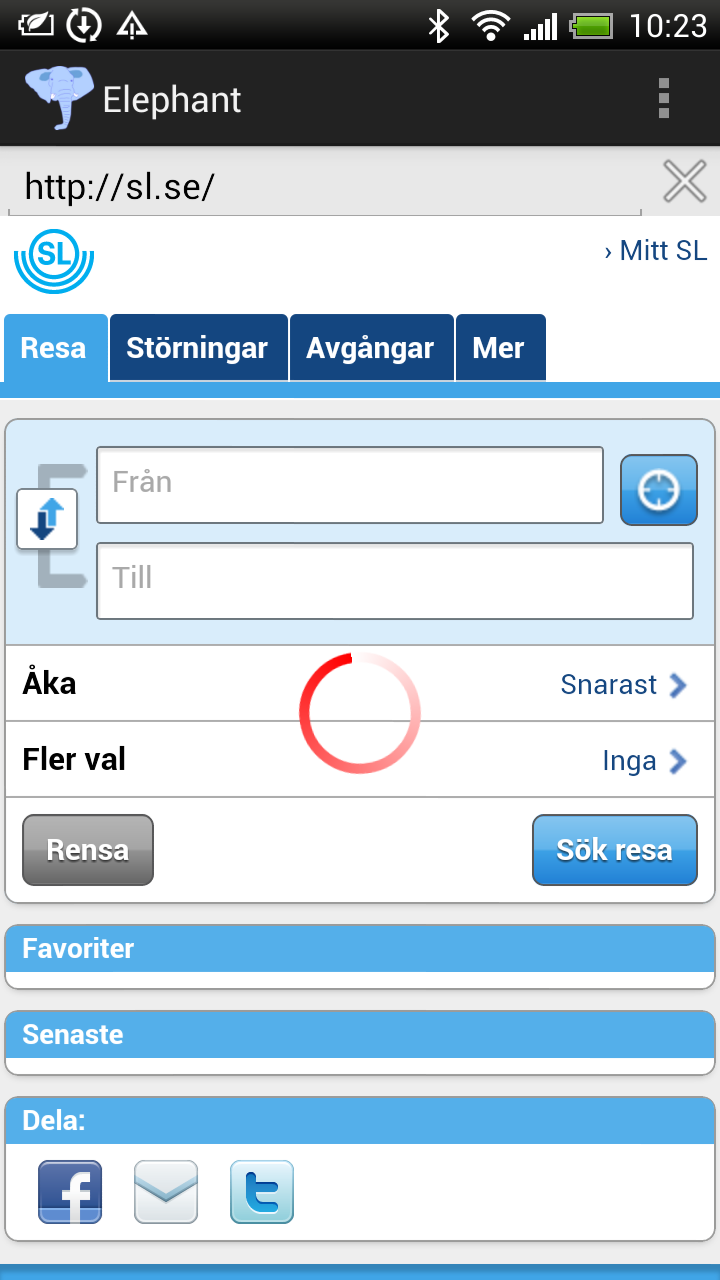
\includegraphics[scale=0.2]{img/loaded_page.png}
\caption{Loading a web page via uplink}\label{fig:loaded_page}
\end{figure}

To make sure that Elephant will be able to retrive resources from an NRS caching node and to be able
to connect to other devices via Bluetooth, the NetInf Service application has to be up and running.
This because the NetInf Services give support for the comunication to other nodes in the system and keep
track on which devices have a certain resource to serve via Bluetooth.

Elephant contains some customizable settigs that can be found in the menu entry on the top right of the application.
These settings makes it possible to take advantage of the NetInf Services, and make the web browser in some sense
unique in the way it works compared to other web browsers.
Since one the core ideas of Information-Centric Networking is to share content between nodes, the setting page
tries to present a simple and transparent way to exploit the underlying capabilities of the NetInf Services.
The user can decide if she wants to share visited pages, and also if she wants to upload web pages to a cache node.
The first menu entry will publish only the name of the web pages that have been visited and the resources in those
pages to an NRS together with the address of the device that holds the pages. In this way the device that registered
itself as a locator can serve content to other devices via Bluetooth.
Enabling the second menu entry will upload not only the identifiers of the resources, but also the actual bytes,
so that the content can be served by an NRS cache node if there is one available.

The last menu entry is for opening the NetInf Services' settings, so that the user does not have to switch application
manually for changing the setting of the services. \\

\begin{figure}[!h]
\centering
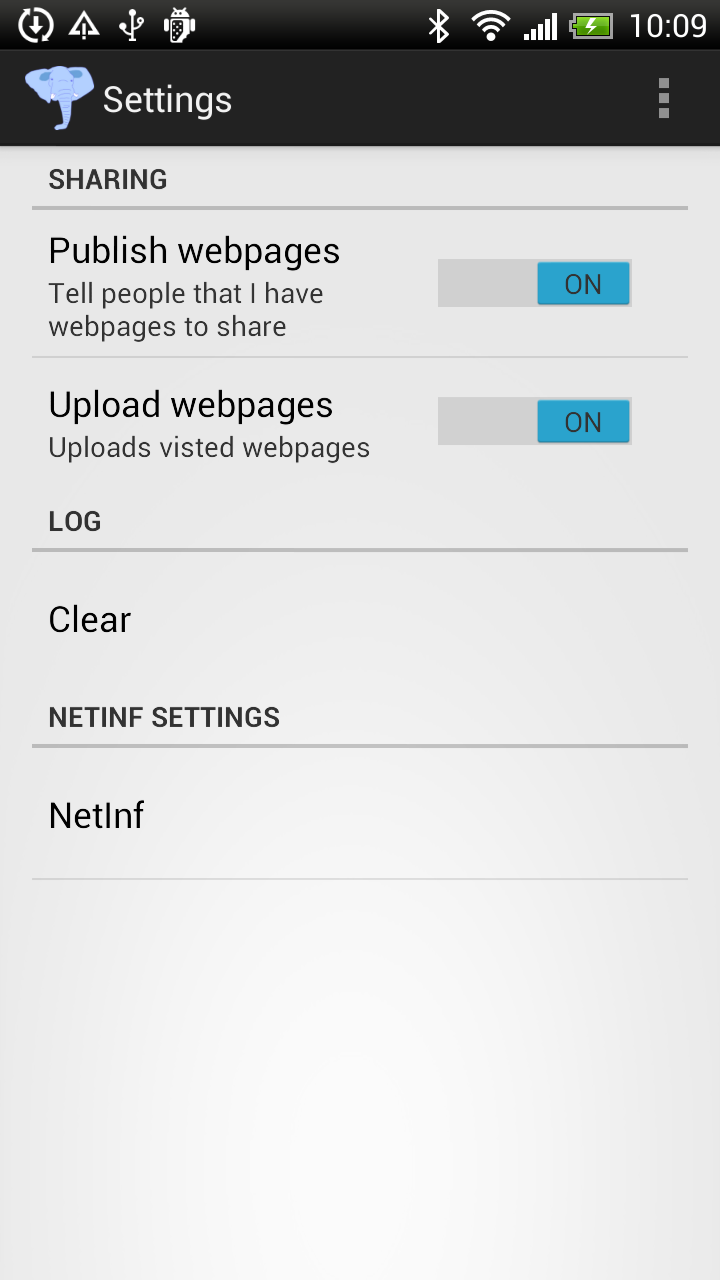
\includegraphics[scale=0.2]{img/ele_settings.png}
\caption{Settings view of Elephant}\label{fig:ele_settings}
\end{figure}


\subsection{NetInf Service}
